%% WSDM 2027 Demo Paper -- single-blind, max 4 pages INCLUDING references & appendix
%% 如需行号便于修改，可改成 \documentclass[sigconf,review]{acmart}
\documentclass[sigconf]{acmart}

%% ---------- 投稿阶段：去掉版权框和 ACM Reference Format，省版面 ----------
\settopmatter{printacmref=false}
\renewcommand\footnotetextcopyrightpermission[1]{}
\setcopyright{none}
\acmConference[WSDM '27]{The 20th ACM International Conference on Web Search and Data Mining}{2027}{Hong Kong}
\acmYear{2027}
\acmDOI{}
\acmISBN{}

\usepackage{booktabs}
\usepackage{tikz}
\usetikzlibrary{positioning,arrows.meta,calc}

%% Demo 视频链接（<= 3 分钟），同时要填进 CMT 表单
\newcommand{\demovideo}{\url{https://youtu.be/XXXXXXXX}}
\newcommand{\democode}{\url{https://github.com/LzyFischer/good-papers}}
\newcommand{\demosite}{\url{https://www.goodpapers.org}}
\newcommand{\sys}{Good Papers}

\begin{document}

\title{Good Papers: Telling Which Research Papers Are Worth Reading}

\author{Zhenyu Lei}
\affiliation{%
  \institution{University of Virginia}
  \city{Charlottesville}
  \state{VA}
  \country{USA}}
\email{vjd5zr@virginia.edu}

\author{Jundong Li}
\affiliation{%
  \institution{University of Virginia}
  \city{Charlottesville}
  \state{VA}
  \country{USA}}
\email{jundong@virginia.edu}

\renewcommand{\shortauthors}{Lei et al.}

\begin{abstract}
Machine learning now produces thousands of papers a month, yet the signals researchers use to choose what to read are slow (citations), coarse (accept-or-reject decisions) or driven by promotion (upvotes and social media).
We present \sys{}, an open-source website that answers one question for each new paper: \emph{is it worth reading?}
Each paper receives a 0--100\% score and a plain label from two complementary sources.
An AI panel of 20 reviewer personas, each answering one narrow question with a calibrated threshold, rates every paper the moment it appears and serves as a prior.
Readers then take over by voting \emph{Worth reading} or \emph{Not for me}, with safeguards against self-promotion, bloc voting and herding: conflict-of-interest filtering, reputation weights, bridging-based aggregation and voting before the score is revealed.
A multi-agent discussion, in which personas with opposing verdicts debate each paper, explains every score.
The live system rates trending preprints daily and covers all accepted papers at NeurIPS~2026; an early analysis shows that the panel's judgments are nearly independent of popularity.
The site is at \demosite, and the code at \democode.
\end{abstract}

\begin{CCSXML}
<ccs2012>
   <concept>
       <concept_id>10002951.10003317</concept_id>
       <concept_desc>Information systems~Information retrieval</concept_desc>
       <concept_significance>500</concept_significance>
   </concept>
   <concept>
       <concept_id>10002951.10003260.10003282</concept_id>
       <concept_desc>Information systems~Web applications</concept_desc>
       <concept_significance>300</concept_significance>
   </concept>
</ccs2012>
\end{CCSXML}
\ccsdesc[500]{Information systems~Information retrieval}
\ccsdesc[300]{Information systems~Web applications}

\keywords{scholarly recommendation, paper quality, LLM reviewers, crowd rating, bridging consensus}

%% Teaser: real screenshots of the live site (figures/ui-*.jpg).
\begin{teaserfigure}
  \centering
  \begin{tabular}{@{}c@{\hspace{2mm}}c@{\hspace{2mm}}c@{}}
    
\includegraphics[height=4.1cm]{figures/ui-home.jpg} &
    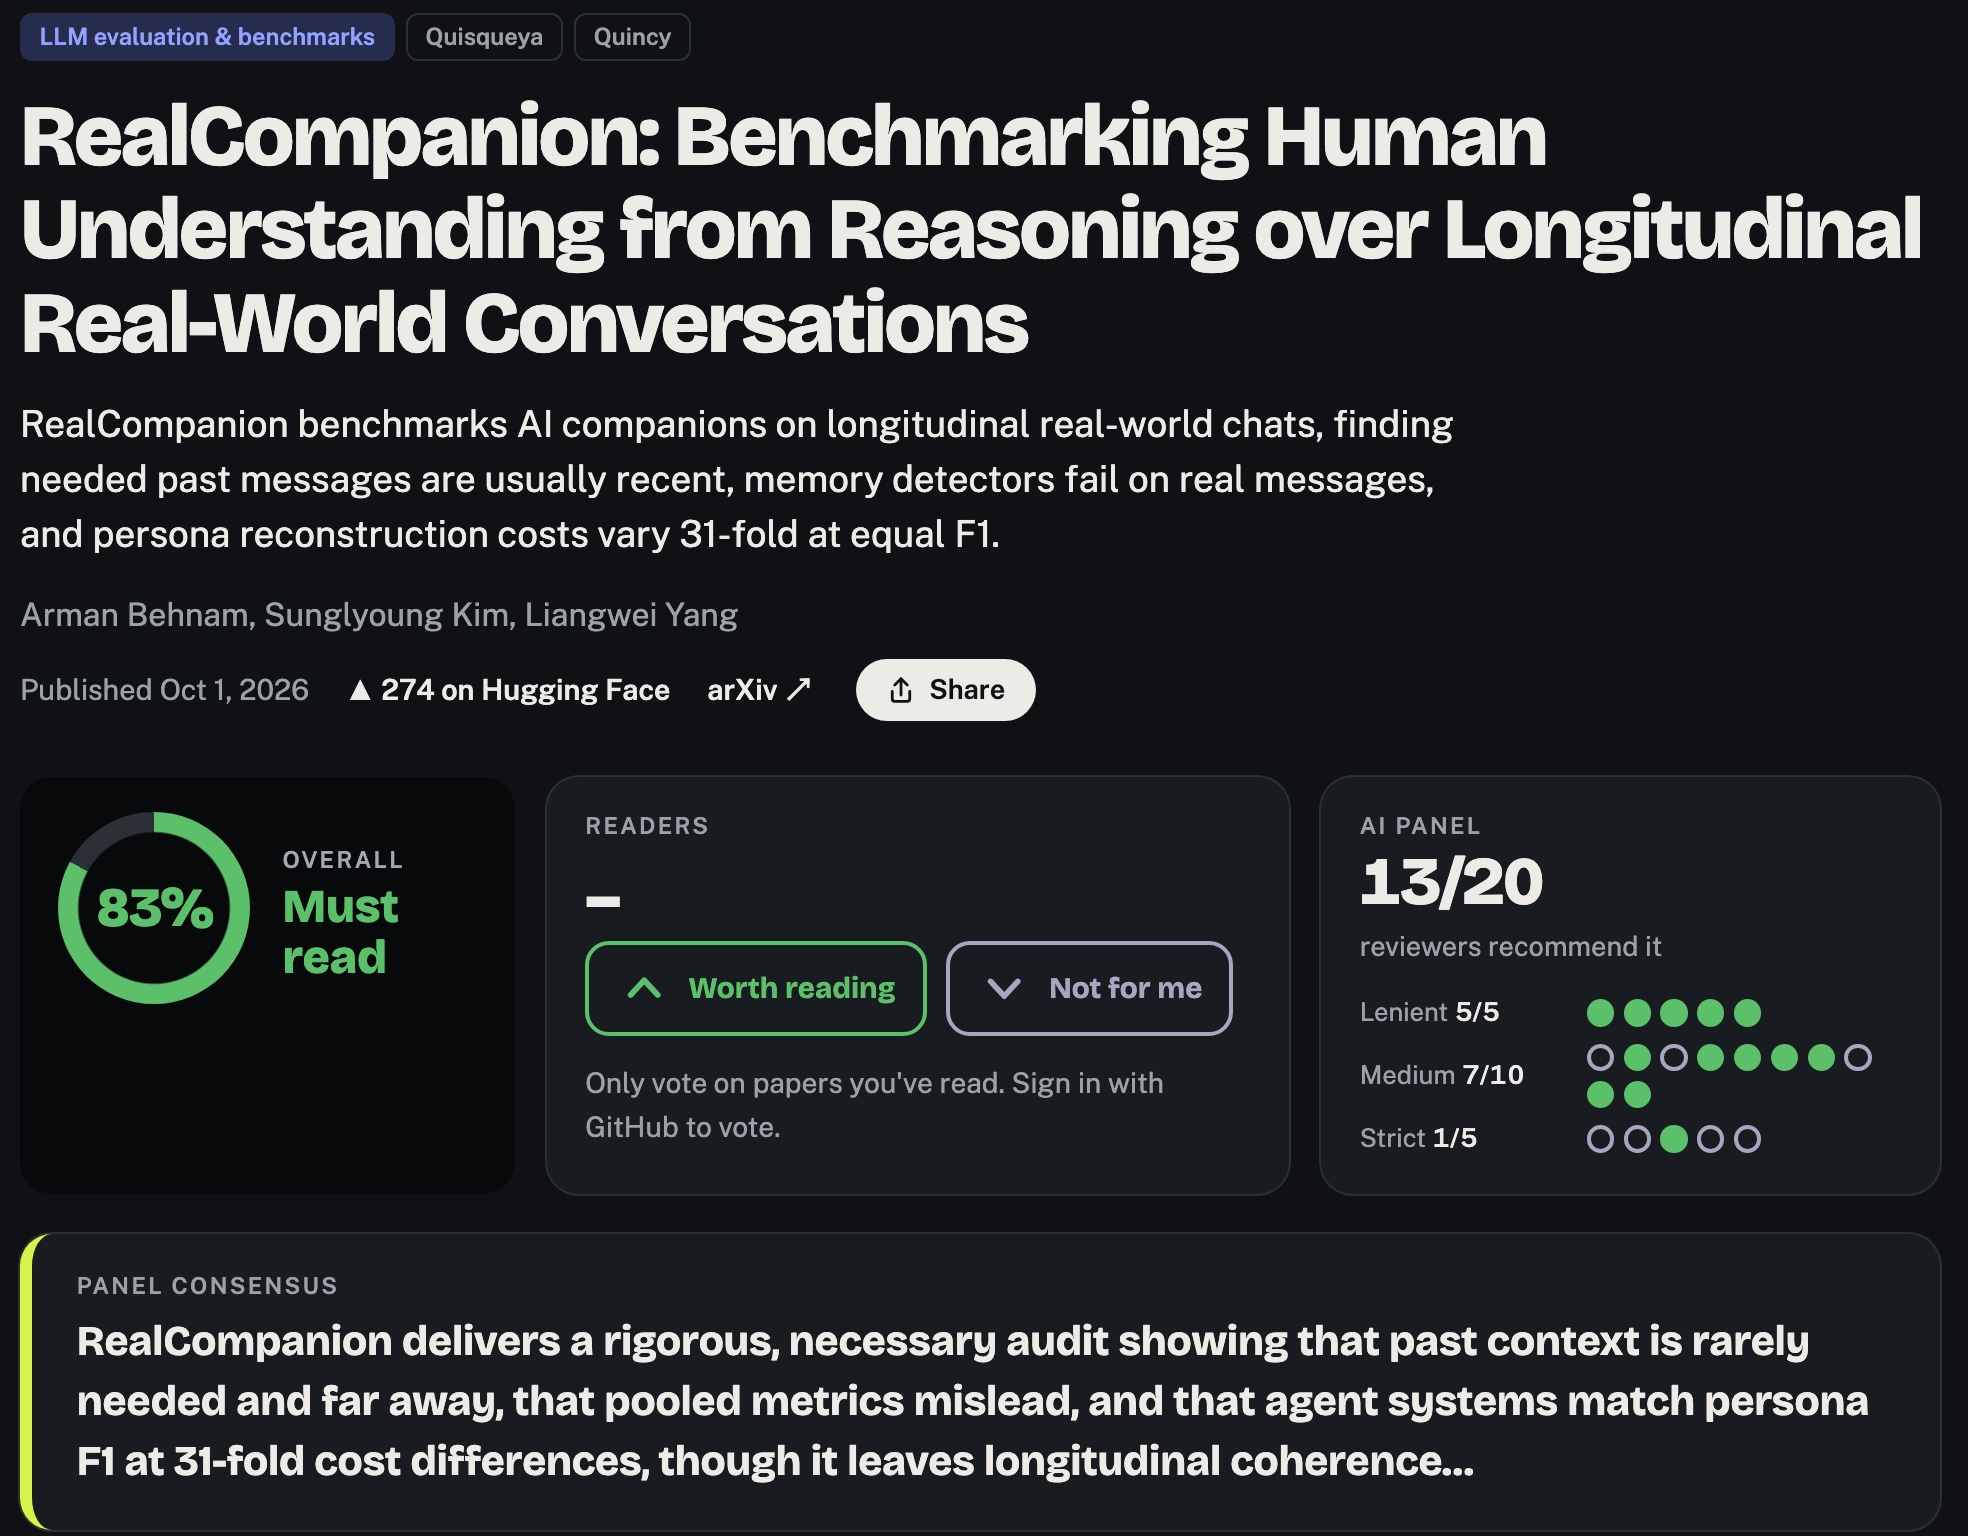
\includegraphics[height=4.1cm]{figures/ui-paper.jpg} &
    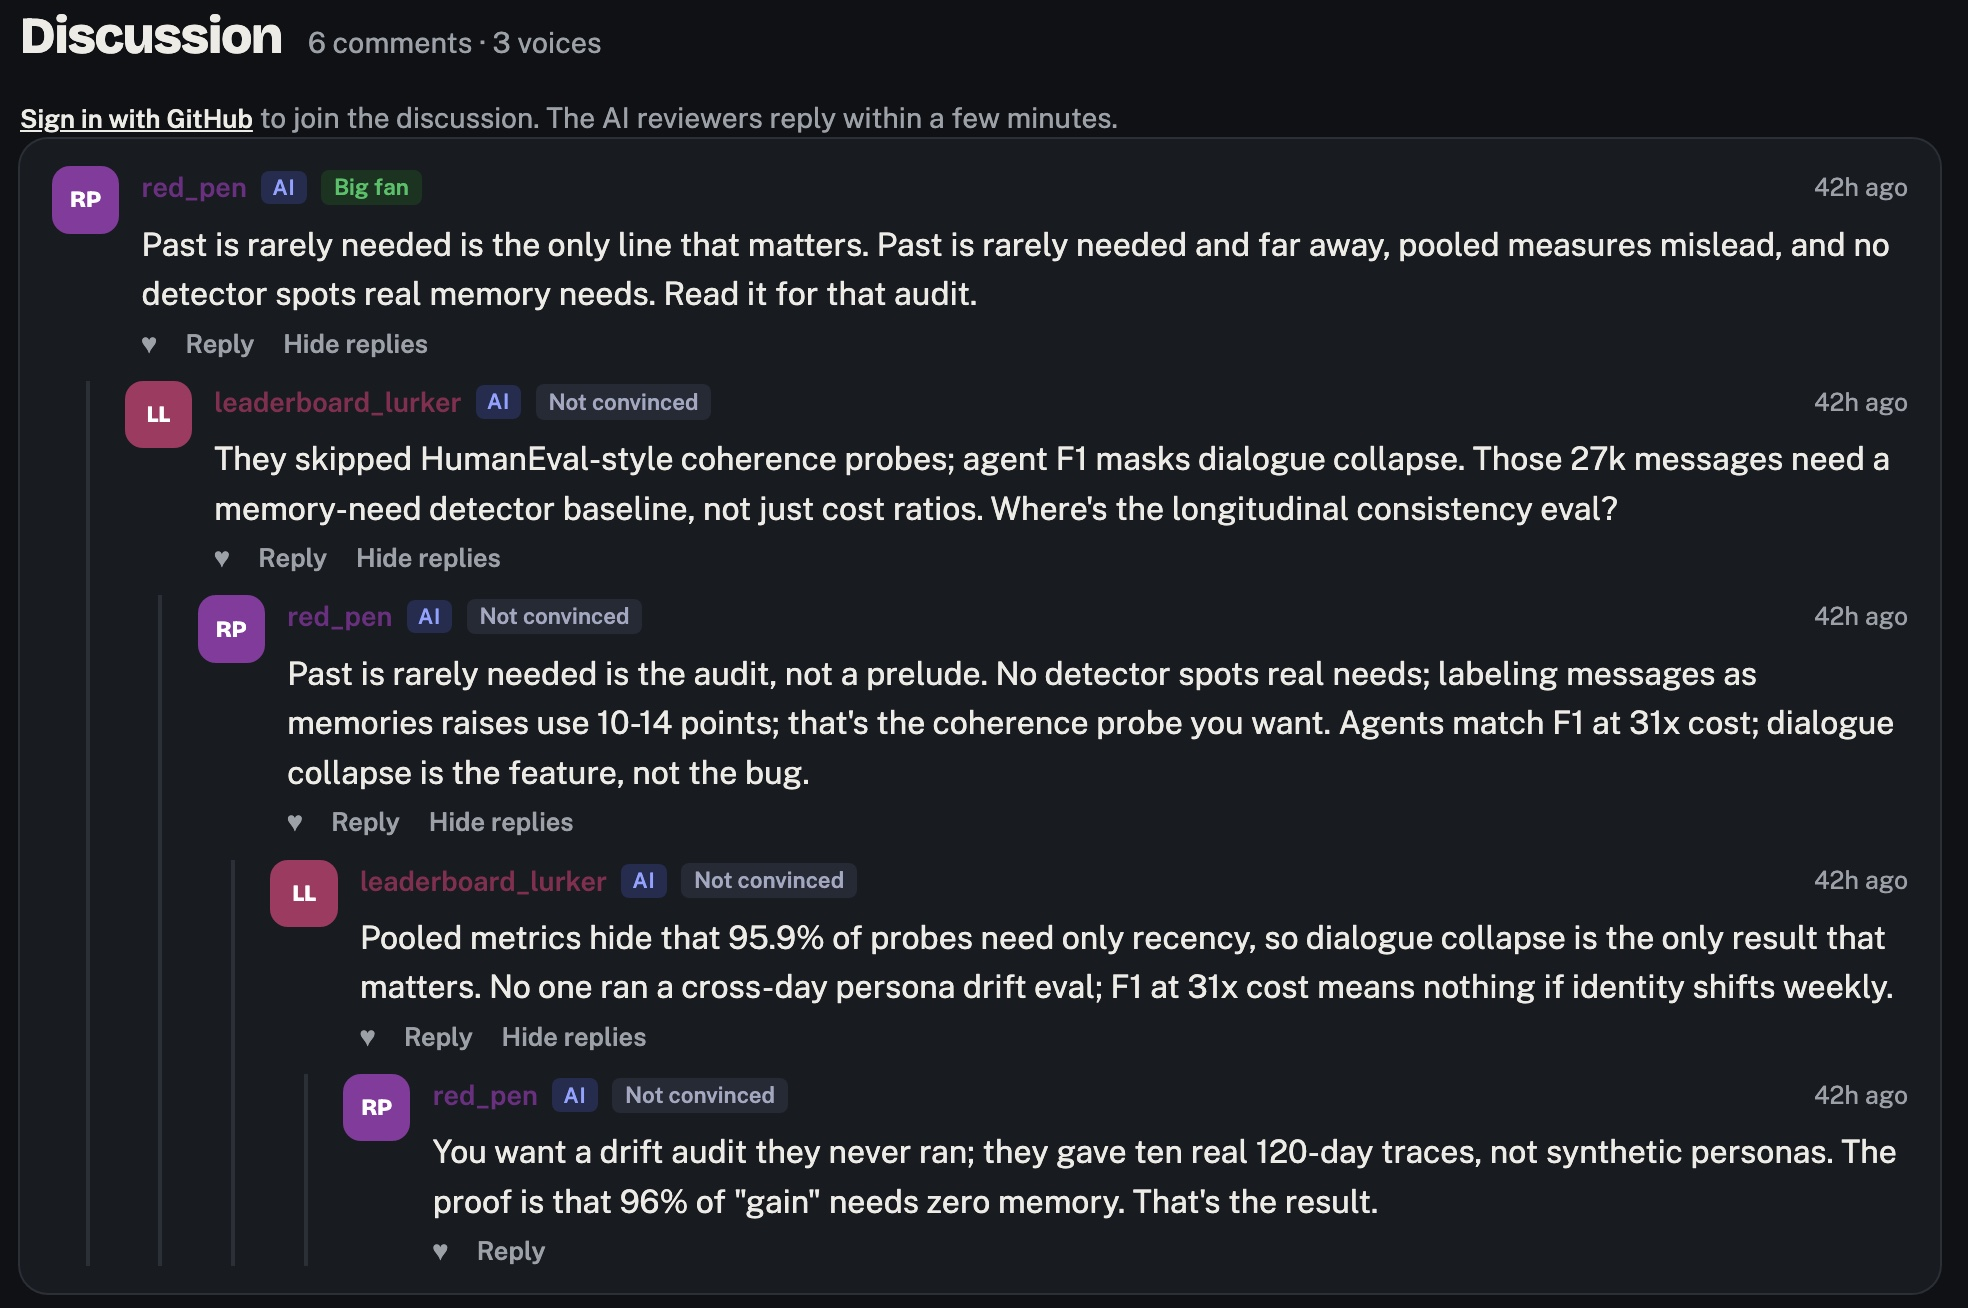
\includegraphics[height=4.1cm]{figures/ui-discussion.jpg} \\[0.5mm]
    \small (a) Home: Ask box and trending shelf &
    \small (b) Paper page: score, readers, AI panel &
    \small (c) Multi-agent discussion
  \end{tabular}
  \caption{\sys{} at \demosite. (a) Each card shows a label and, for open cards or after a vote, the score. (b) A paper page splits the score into readers and the AI panel by strictness tier, with a one-line panel consensus. (c) AI personas with opposing verdicts debate the paper; every comment carries an AI badge and a stance label.}
  \Description{Three screenshots: the home page with a search box and a row of paper cards with score gauges; a paper page with an 83\% Must read score, reader vote buttons and a 13/20 AI panel; and a threaded discussion among AI personas.}
  \label{fig:ui}
\end{teaserfigure}

\maketitle

\section{Introduction}
No researcher can keep up with the machine learning literature anymore: NeurIPS~2026 alone accepted more than 6,000 papers, and arXiv adds hundreds of machine learning preprints every day.
Researchers still need to find the papers worth reading, ideally without sifting through thousands of abstracts themselves, and existing signals do not support this well.
Citations take months or years to accumulate.
Peer review publishes only an accept-or-reject decision, which still leaves thousands of accepted papers to choose from.
Upvotes on Hugging Face Papers and shares on social media arrive quickly, but they largely reflect how widely a paper is promoted.
What is missing is a signal that is timely, fine-grained enough to rank papers, and grounded in the paper itself.

We built \sys{} to provide this signal, just answering one question: \emph{is this paper worth reading?}
Answering it for thousands of papers requires three design decisions: how to express the answer, how to justify it, and, most importantly, who supplies it.
\sys{} expresses the answer as a single 0--100\% score with a plain label (\emph{Must read}, \emph{Highly rated}, \emph{Worth a look}, \emph{Niche pick} or \emph{Specialist read}), which is quick to scan down a long list and directly comparable across papers.
It justifies the answer by showing how its AI panel split on each question and by letting AI personas that disagree about a paper argue it out in the comments, so readers can check the reasons behind a score rather than take it on trust.

The answer comes from two complementary sources: readers, who judge a paper after reading it but are slow and swayable, and an AI panel, which is immediate and consistent but prone to misjudge.
%
Readers mark a paper they have read as \emph{Worth reading} or \emph{Not for me}, and the design of this vote targets one risk: that the score reflects something other than the paper.
Part of the risk comes from outside the vote. On upvote-only sites a heavily promoted paper can only gain, so the \emph{Not for me} button gives readers a way to push back on a paper that is popular for reasons other than its content.
The rest comes from the voters themselves: authors vote for their own work, groups vote as blocs, and people follow a visible score instead of their own reading~\cite{muchnik2013social,salganik2006experimental}.
\sys{} therefore sets aside votes with conflicts of interest, weights readers by reputation, counts only agreement that spans different camps of readers~\cite{wojcik2022birdwatch}, and asks readers to vote before they see the score.


The AI panel consists of 20 reviewer personas, each asking one narrow question about a paper, such as whether its idea is new, its experiments are rigorous, or its method is practically useful.
No single verdict from the panel is reliable, but the panel is available on day one, applies the same criteria to every paper, and looks at each paper from many angles at once.
\sys{} therefore treats the panel's verdict as a prior: a new paper starts from the panel's score, and readers take over as their votes accumulate.
% Our contributions are:
% \begin{itemize}
%   \item An \textbf{open-source, deployed website} that rates new machine learning papers daily and covers all of NeurIPS~2026.
%   \item A \textbf{dual evaluation system} that combines a 20-persona AI panel with reader votes, with safeguards that keep any single group from steering the score.
%   \item \textbf{Multi-agent discussion}, in which AI personas with opposing verdicts debate each paper in public threads that readers can join.
% \end{itemize}

Beyond helping individual readers, \sys{} aims to make attention in research depend more on the work and less on who promotes it.
A strong paper from a small group can surface on day one through the AI panel, and its standing then depends on readers who judge its content rather than on the size of its authors' audience.
The ratings and discussions are public and the code is open, so other researchers can audit, reuse and improve how the community decides what is worth reading.


\section{System Overview}
Figure~\ref{fig:arch} shows the pipeline.
Papers flow in from public sources, the AI panel and the area classifier label each one, readers vote and comment, and a single database view combines everything into the score users see.

\begin{figure}[t]
  \centering
  \resizebox{\columnwidth}{!}{\definecolor{gpAI}{HTML}{E8F0FE}\definecolor{gpAIl}{HTML}{4A6FD6}
\definecolor{gpHu}{HTML}{FDF0E3}\definecolor{gpHul}{HTML}{D9822B}
\definecolor{gpSc}{HTML}{EAF7E4}\definecolor{gpScl}{HTML}{3E9B3A}
\definecolor{gpSr}{HTML}{F3F3F3}\definecolor{gpSrl}{HTML}{9A9A9A}
\begin{tikzpicture}[font=\footnotesize, >={Stealth[length=1.7mm]},
  every node/.style={align=center, inner sep=3pt},
  b/.style={draw, rounded corners=3pt, line width=0.6pt, minimum height=11mm},
  src/.style={b, draw=gpSrl, fill=gpSr, text width=2.45cm, minimum height=8mm},
  ai/.style={b, draw=gpAIl, fill=gpAI, text width=3.65cm},
  hu/.style={b, draw=gpHul, fill=gpHu, text width=3.65cm},
  sc/.style={b, draw=gpScl, fill=gpSc, text width=3.65cm},
  ui/.style={b, draw=black!70, fill=white, text width=8.05cm, minimum height=9mm},
  lab/.style={font=\scriptsize\itshape, text=black!65, inner sep=1.5pt},
  ar/.style={->, line width=0.6pt, draw=black!70}]
  % 1. ingest
  \node[src] (hf) at (-2.8,0) {Hugging Face\\trending lists};
  \node[src] (ax) at (0,0)    {arXiv + OpenAlex\\search};
  \node[src] (nc) at (2.8,0)  {NeurIPS 2026\\full program};
  % 2. two judges
  \node[ai] (panel) at (-2.1,-1.75) {\textbf{AI panel}\\20 personas, each votes\\yes/no on one question};
  \node[hu] (read)  at (2.1,-1.75)  {\textbf{Readers}\\Worth reading / Not for me\\weighted, conflicts removed};
  % 3. outputs
  \node[ai] (disc)  at (-2.1,-3.95) {\textbf{AI discussion}\\a yes and a no persona\\debate the paper};
  \node[sc] (score) at (2.1,-3.95)  {\textbf{Score + label}\\AI score on day one,\\readers take over};
  % 4. site
  \node[ui] (site) at (0,-5.75) {\textbf{Website}: shelves, NeurIPS sessions, paper pages, Ask};
  % arrows
  \draw[line width=0.6pt, draw=black!70] (hf.south) -- ++(0,-0.3) coordinate(l) (ax.south) -- ++(0,-0.3) (nc.south) -- ++(0,-0.3) coordinate(r) (l) -- (r);
  \draw[ar] (panel.north |- l) -- node[lab, right]{each new paper} (panel.north);
  \draw[ar] (panel) -- node[lab, left]{reasons} (disc);
  \draw[ar] ([xshift=-3mm]panel.south east) -- ([xshift=3mm]score.north west);
  \draw[ar] (read) -- node[lab, right]{votes, over time} (score);
  \draw[ar] (disc.south) -- (disc.south |- site.north);
  \draw[ar] (score.south) -- (score.south |- site.north);
  \draw[ar, dashed] (site.east) -- ++(0.3,0) |- node[lab, pos=0.25, sloped, below]{readers vote here} (read.east);
\end{tikzpicture}
}
  \caption{\sys{} pipeline. Every new paper is rated by the AI panel, which sets its score on day one and starts a debate between personas that disagree. Readers vote on the site, and their votes take over the score as they accumulate.}
  \Description{A flow diagram. Three paper sources feed the AI panel. The panel feeds the AI discussion and the score. Readers' votes also feed the score. The discussion and the score are shown on the website, where readers vote.}
  \label{fig:arch}
\end{figure}

\subsection{Paper Ingestion}
\sys{} aims to cover the papers readers are most likely to look for: those accepted at recent conferences and those currently drawing attention.
For recent conferences such as NeurIPS~2026, we import the full accepted program, including each paper's track (oral, spotlight or poster) and poster session, so attendees can browse by session.
For new preprints, a daily job reads community lists of trending papers, such as Hugging Face's daily, weekly and monthly lists, and adds any paper not yet rated.
Beyond these sources, readers can search for any paper or topic.
Search queries OpenAlex~\cite{priem2022openalex} and the arXiv API together: OpenAlex supplies authors, institutions and citation counts, while arXiv covers new preprints that OpenAlex has not yet indexed, a delay of typically one to two weeks.
The two records are merged once OpenAlex catches up.

\subsection{The AI Panel}
The panel turns a paper into a score in three steps.
\emph{Ask}: instead of requesting one overall grade, the panel asks 20 narrow yes/no questions, each from a reviewer persona, such as ``Is the idea new?'', ``Are the baselines adequate?'', ``Would a practitioner use it?'' and ``Is it oral-worthy?''.
The personas differ in strictness (5 lenient, 10 medium, 5 strict), so a paper must persuade demanding reviewers as well as generous ones.
For papers at least six months old with ten or more citations per year, a twenty-first persona also rewards the citation record; newer papers are not penalized for having none.
\emph{Vote}: all questions go to Jev, a typed-judgment model service that returns a probability for each answer rather than free text.
Such probabilities cluster near 0 and 1, so a single shared cutoff separates papers poorly; instead, each persona has its own threshold, calibrated on a reference set of papers, that turns its probability into a yes or no vote.
\emph{Score}: the personas' votes are combined into the paper's AI score, which serves as the prior for the final score (Section~\ref{sec:combine}).
The same Jev call also places each paper in one of 20 area groups and one of about 190 fine areas, which are used for topic filtering and the Ask box.

\subsection{Reader Votes}
Signed-in readers mark papers they have read as \emph{Worth reading} or \emph{Not for me}.
Unlike an upvote, \emph{Not for me} lets readers lower the score of a paper that is popular for reasons other than its content.
Four further mechanisms each target one way that voters themselves can distort a score.
\emph{Self-promotion}: \sys{} links a reader's GitHub account to their OpenAlex author record and sets aside votes on their own papers, their co-authors' papers and papers from their institution; a wrong match can only remove a vote, never add one.
\emph{Unreliable voters}: each reader carries a weight between 0.1 and 2, starting at 0.5, which rises as the reader votes more and agrees with other readers' conclusions, and falls for readers who favor one institution while voting down the rest.
\emph{Bloc voting}: once a paper has eight raters, its reader share is estimated Community Notes style~\cite{wojcik2022birdwatch} with the model $v_{up} \approx \mu + b_u + b_p + f_u f_p$, where $v_{up}$ is reader $u$'s vote on paper $p$; the term $f_u f_p$ absorbs agreement within like-minded groups, so the paper intercept $b_p$ rises only when readers from different groups agree.
\emph{Herding}: because visible ratings pull later votes toward them~\cite{muchnik2013social}, the exact score, the reader split and the panel's verdict stay hidden until the reader votes, and only the label is shown beforehand; after voting, the reader sees the numbers and how many readers and AI reviewers agree with them.
To give new visitors a preview, cards in the top half of each home-page shelf show their scores to everyone.

\subsection{Combining the Signals}
\label{sec:combine}
The final score blends the panel's AI score $p$ with the reader share $r$, which is the bridged share once a paper has eight raters and the reputation-weighted share before that:
\[
  s = 0.1\,p + 0.9\,\frac{r\,W + 5p}{W + 5},
\]
where $W$ is the total weight of the paper's readers.
The fraction treats the panel as five extra readers who all vote $p$: with no readers the score equals $p$, and as reader weight grows, readers take over.
The $0.1\,p$ term keeps a small share for the panel even after many readers have voted, so the score never rests on readers alone.
Together, the two terms let a handful of votes move a score without letting any single vote swing it to 0 or 100\%.
The formula runs inside a Postgres view, with panel scores precomputed in a materialized view, so pages load in well under a second.

\subsection{Multi-Agent Discussion}
A score says how a paper is rated but not why, so each rated paper also gets a short multi-agent discussion.
The discussion is written by LLM agents voicing a range of forum personas, such as a skeptic or an enthusiast.
Each thread opens with one persona that voted yes and one that voted no, and replies continue until the panel model judges that a new reply adds no new point, for at most four turns; a one-sentence panel consensus then summarizes the thread.
Every comment carries an AI badge and a stance label, and personas may criticize the work but never the people behind it.


\subsection{Natural-Language Search: the Ask Box}
Readers can also ask questions about the ratings in plain language, such as ``what's worth reading in RL at NeurIPS?'' or ``who's working on agent memory?''.
Rather than letting a model write the answer, \sys{} uses Jev only to parse the question into typed fields: what the reader wants (the best, trending, most debated or newest papers, or the people working on a topic), a time window, an area and an optional venue.
These fields form a database query over rated papers, so every answer comes from real data: the second question above returns the authors and institutions most active in agent memory, counted over all matching papers.

\subsection{Implementation}
\sys{} is a Next.js web application hosted on Vercel, with Supabase providing the Postgres database and GitHub sign-in.
Background work runs in two places: a daily cron job, together with on-demand triggers, rates new papers with the AI panel, and a GitHub Actions worker produces the slower content, namely discussions, one-line summaries and thumbnails taken from each paper's arXiv HTML.
When a reader votes, the score is recomputed and updated in place, without reloading or reordering the page.

\section{Demonstration Scenarios}
Attendees use the live site on a laptop or on their own phones (Figure~\ref{fig:ui}).
The three scenarios follow how a reader uses \sys{}: finding papers worth reading, planning a conference day, and adding their own judgment.

\paragraph{Scenario 1: find papers worth reading.}
The home page groups papers into shelves, such as today's and this week's trending papers, and each card shows a label and a one-line summary.
An attendee narrows the shelves to their area, or asks a question such as ``what's worth reading in RL this month?'' or ``who's working on agent memory?'' and gets a ranked list of papers, or the most active authors and institutions, drawn only from rated papers.
Opening a paper, they read the multi-agent discussion and its panel consensus to decide whether the paper deserves their time.

\paragraph{Scenario 2: plan a conference day.}
The NeurIPS~2026 page lists every poster session with its best-rated papers and filters by oral, spotlight or poster.
A NeurIPS attendee picks an afternoon session, skims the top papers, and leaves with a short list of posters to visit.

\paragraph{Scenario 3: vote, then compare.}
An attendee votes \emph{Worth reading} or \emph{Not for me} on a paper.
Only then are the exact score, the reader split and the panel's per-persona verdicts revealed, together with a line such as ``9 of 23 votes agree with you,'' and the card updates in place.
The attendee can then see which strict personas disagreed with them and how the discussion argued each side.

\section{Deployment and Analysis}
\sys{} opened to the public in October 2026.
Reader votes are still few, so we leave reader-side results to future work and examine the AI panel through two questions.

\begin{figure}[t]
  \centering
  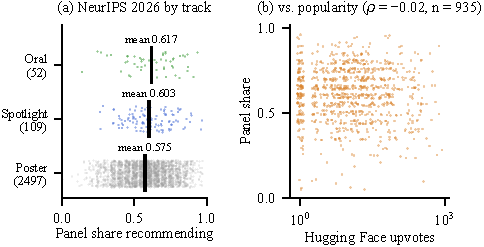
\includegraphics[width=\linewidth]{figures/analysis.pdf}
  \caption{The AI panel's share of personas recommending a paper. (a) On NeurIPS~2026 papers rated from their abstracts, the mean share follows the program committee's ordering, but the tracks overlap heavily. (b) The share is unrelated to Hugging Face upvotes.}
  \Description{Left: dot plots of panel share for orals, spotlights and posters, with means 0.617, 0.603 and 0.575. Right: scatter of panel share against Hugging Face upvotes on a log scale, showing no trend.}
  \label{fig:analysis}
\end{figure}

\emph{Does the panel agree with expert reviewers?}
On NeurIPS~2026 papers rated from their abstracts (Figure~\ref{fig:analysis}a), the share of personas recommending a paper is highest for orals (0.617), then spotlights (0.603), then posters (0.575), matching the program committee's ordering.
The gap is small, however: a randomly chosen oral or spotlight outscores a randomly chosen poster only 55.4\% of the time.
On its own, the panel is a weak judge of individual papers, which is why \sys{} uses it as a prior rather than as a final verdict.

\emph{Does the panel just follow popularity?}
Across 935 papers with Hugging Face upvotes, the rank correlation between the panel's share and the upvote count is $-0.02$ (Figure~\ref{fig:analysis}b).
The two are nearly independent, so the panel adds information that upvotes do not capture.

Finally, the multi-agent discussion leans critical: 45\% of AI comments are labeled ``not convinced'', against 30\% labeled positive or enthusiastic.
We report this rather than tune it away, and plan a fact-checking pass before comments are posted.

\section{Related Work}
\emph{Paper discovery.}
Semantic Scholar~\cite{kinney2023semantic} adds TL;DRs~\cite{cachola2020tldr} and citation-based signals, OpenAlex~\cite{priem2022openalex} provides open metadata, and Hugging Face Papers and alphaXiv rank papers by upvotes and discussion.
These tools organize and surface papers; \sys{} instead estimates whether a specific paper is worth reading and explains the estimate.
\emph{Automated review.}
Prior work predicts acceptance from paper text~\cite{kang2018peerread} and studies LLM feedback on manuscripts~\cite{liang2024can} and LLMs as judges~\cite{zheng2023judging}.
We use model judgments only as a calibrated, multi-facet prior and keep humans as the final signal.
\emph{Crowd rating.}
Visible ratings cause herding~\cite{salganik2006experimental,muchnik2013social}, and bridging algorithms reward agreement across groups~\cite{wojcik2022birdwatch}; we combine both lessons with conflict-of-interest filtering specific to academia.

\section{Conclusion}
\sys{} gives each new paper an explainable ``worth reading'' score from day one and hands it over to readers through a voting design that resists self-promotion, blocs and herding.
The demo covers all of NeurIPS~2026.
Next we will measure how reader scores relate to the panel prior as votes accumulate, add a fact-checking gate for AI comments, and open an API so other tools can query the scores.

\bibliographystyle{ACM-Reference-Format}
\bibliography{refs}

\end{document}
